\documentclass{article}

\usepackage{amsmath} % For gather and other math environments
\usepackage{setspace} % For double spacing
\usepackage{mathtools} % amsmath extensions
\usepackage{amsfonts} % math fonts
\usepackage{graphicx} % for images
\usepackage{listings} % for code blocks
\usepackage{pgfplots}

\usepackage[a4paper, margin=3.17cm]{geometry}

\graphicspath{{ ./images/ }}

% notes:
% https://hudsonthames.org/caveats-in-calibrating-the-ou-process/
% closed-form OU solution, do this youself tho: https://fxpaul.wordpress.com/2011/05/27/closed-form-solution-of-modified-ornstein-uhlenbeck-process/
% interesting: https://arxiv.org/pdf/2003.10502
% https://github.com/david-alber/Pairs-Trading-as-application-to-the-Ornstein-Uhlenbeck-Process

% process calibration:
% https://dr.lib.iastate.edu/entities/publication/bf86f169-61a5-44fc-8f2f-d8e6cd7e103a

% out-of-sample performance of an OU process:
% https://onlinelibrary.wiley.com/doi/abs/10.1002/for.2720

% maybe I just didn't account for stochastic drift?

% rly interesting:
% https://github.com/david-alber/Pairs-Trading-as-application-to-the-Ornstein-Uhlenbeck-Process/blob/master/Report%2BPoster/Pairs_Trading_Doc.pdf

\begin{document}
\begin{spacing}{2.0}

\section{Brownian Motion and the Wiener Process}

Consider a stochastic process, where per each iteration, we add a $\Delta$ to the previous value,
this $\Delta$ is distributed by a normal distribution with a $mu$ of zero, and these are independent
stochastic events this is called the Wiener process. In discrete time, we can define the Wiener process
with the following equation
\begin{gather*}
    W_{t + 1} = W_{t} + \mathcal{N}(0, \sigma^{2})
\end{gather*}
Where $W_{t + 1}$ is the next value of the process (under discrete time), $\mathcal{N}(0, \sigma^{2})$
is a normally distributed drift variable with the variance $\sigma^{2}$.

Intuitively, the expected value, i.e. the limit of this process as it approaches infinity, should
be zero, since the normal distribution is symmetric. (maybe prove this? Using a limits on the $\mathbb{E}[W]$ and the normal dist)

The spread of the Wiener process grows at a rate of $\sigma_{t} = \sigma \sqrt{t}$, due to each timestep adding additional compounded uncertainty.

Here's an example of a Wiener process with $W_{0} = 0$ and $\sigma^{2} = 1$:
\begin{center}
    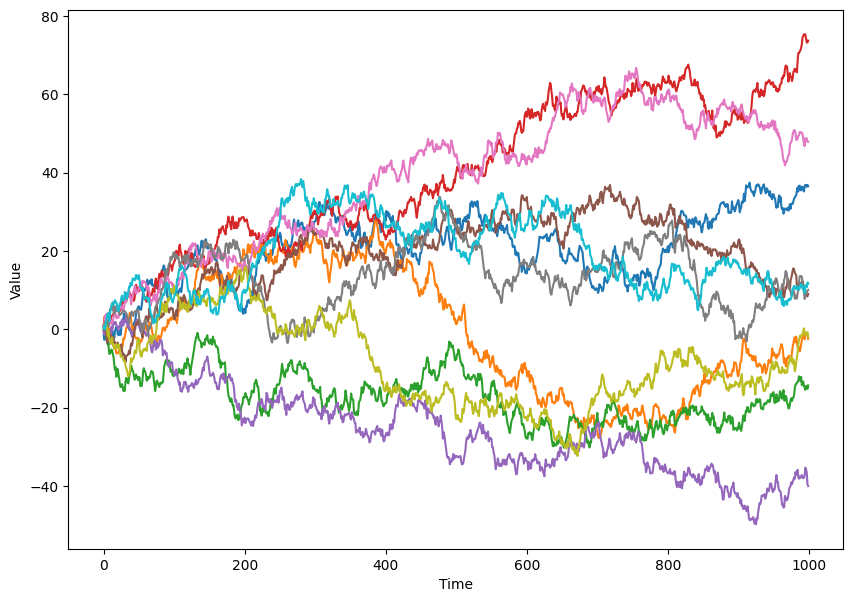
\includegraphics[scale=0.35]{./images/wiener.png}
\end{center}
In the diagram, we can clearly observe that the the variance of the Wiener process gets larger as the time progresses.

The wiener process is crucial and has many financial applications, for example, equity prices under the assumption of the efficient
market hypothesis follow a purely-stochastic Wiener process. This although disregards stochastic drift, which applies directional
pressure on equity prices, i.e., the Wiener process is market-agnostic, and applies to equity which do not follow the upward trend
of the market due to the positive risk-free rate.


\section{Ornstein-Uhlenbeck Process}

\subsection{Deriving a Mean Reversion Mechanism}

But what if we don't want the variance of the process to get larger as time progresses? We call these processes mean-reverting, as in they
tend to revert their values back towards the mean $\mu$. This has numerous financial applications (not to mention its applications outside
of finance), for example: statstical arbitrage, interest rate models, heston model, and mean reverting equities.

So how do we implement mean reversion? We can start by thinking about what mean reversion actually is? Mean reversion is the tendency of a
variable (or usually a stochastic process) to revert back to its long-term mean. If we consider the roots of brownian motion - physics -, we
can consider a mean-reverting term to be similar to a force pushing a particle back towards its mean; note that this doesn't happen
instantaneuously, it happens over a period of time, where the steadyness of this decay is dictated by the rate of mean-reversion, denoted as
$\theta$.

We know that an exponential function with a negative coefficient applied to the exponent will produce a function that will slowly decay.

\begin{center}
\begin{tikzpicture}
    \begin{axis}[
        axis lines = left,
        xlabel = \(x\),
        ylabel = {\(f(x)\)},
    ]
        \addplot [
            domain=0:15,
            samples=100,
            color=red,
        ] {e^(-0.4 * x)};

        \addlegendentry{$f(x) = x_{0} \cdot e^{-\theta x}$}
    \end{axis}
\end{tikzpicture}
\end{center}

But this is not exactly mean reverting, we need to adjust the function to not only have the tendency to approach zero, but rather, the function must approach
the mean. And the function must be applied from any starting point $x_{0}$. Considering that $f(0) = x_{0}$, we can adjust the function and introduce a base
term: $f(x) = x_{0}e^{-\theta x}$, this ensures the initial value is $x_{0}$, since $e^{0} = 1$. Now we have to ensure that the function converges at the mean,
not at zero. Initially, we can try to add a the mean as a constant term, such that $f(x) = \mu + x_{0}e^{-\theta x}$, but when graphing this function, we notice
that we break our first condition - the initial value of the function $f(0)$ is not equal to $x_{0}$. We have to adjust for this in the coefficient of the
exponential term. We notice that the difference between $x_0$ and $f(0)$ is equal to the mean, thus modifying the function to the following will solve our problem:

\begin{gather*}
    f(x) = \mu + (x_{0} - \theta)e^{-\theta x}
\end{gather*}

The function produces the following graph, assuming $\mu = 4$, $\theta = 0.4$ and varying the initial value $x_{0}$ to be $x_{0} \in \{8, 5, -1 \} $ for each of the
separate lines respectivelly:

\begin{center}
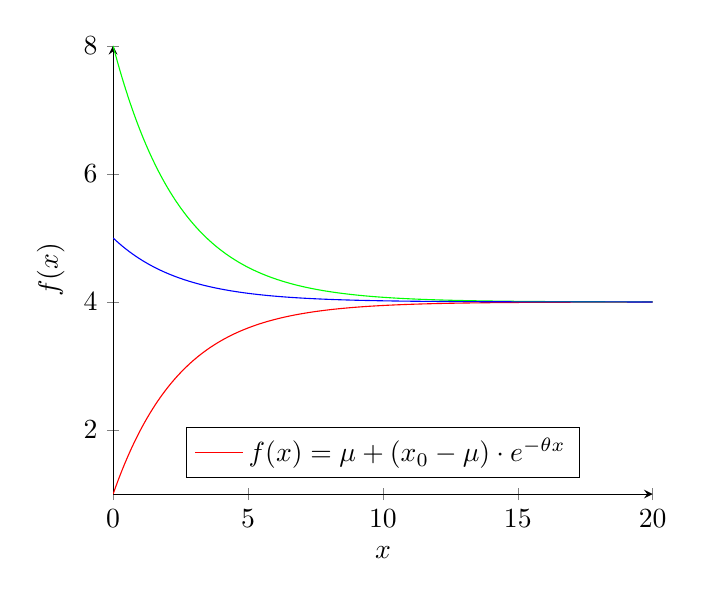
\begin{tikzpicture}
    \begin{axis}[
        axis lines = left,
        xlabel = \(x\),
        ylabel = {\(f(x)\)},
        legend style={
            at={(0.5,0.15)},
            anchor=north,
            cells={anchor=west}
        },
    ]
        \addplot [
            domain=0:20,
            samples=400,
            color=red,
        ] {4 + (1 - 4) * e^(-0.4 * x)};

        \addplot [
            domain=0:20,
            samples=400,
            color=green,
        ] {4 + (8 - 4) * e^(-0.4 * x)};

        \addplot [
            domain=0:20,
            samples=400,
            color=blue,
        ] {4 + (5 - 4) * e^(-0.4 * x)};

        \addlegendentry{$f(x) = \mu + (x_{0} - \mu) \cdot e^{-\theta x}$}
    \end{axis}
\end{tikzpicture}
\end{center}

\subsection{Differentiating for the Mean-reverting Force}

We can now think about creating a stochastic process that will take the Wiener process as a basis, but add mean-reverting properties in order to ensure
the variance stays within a certain range. Just adding a term for the brownian motion will not be enough, this would be misinterpreting the mean-reverting
effect and would be mostly useless for our purposses, thus we can't do something like:
\begin{gather*}
    X_{t} = \mu + (X_{0} - \mu) \cdot e^{-\theta t} + \sigma W_{t}
\end{gather*}
We must now calculate the tug or the actual amount by which the function changes per unit $t$. This will be necessary for our stochastic process, as they
are inherently defined in differential form (in descrete time), where the next value depends on the previous value and we simply add a modifying term, e.g.
$M_{t + 1} = M_{t} + \sigma$. We can do this by taking a simple derivative of the function. This derivative can then be thought of as the per-unit $t$ amount
of tug applied for each value above or below the mean.
\begin{gather*}
    \frac{d}{dt} \left ( \mu + \left ( X_{0} - \mu \right ) \cdot e^{-\theta t} \right ) \\
    \frac{d}{dt} \mu + \frac{d}{dt} \left ( X_{0} - \mu \right ) e^{-\theta t}
\end{gather*}
We know that the derivative of the constant $\mu$ is zero, thus we can eliminate the term. We are left with the derivative of a product, for which we can
use the product rule of differentiation: $\frac{d}{dt}x \cdot y = x'y + xy'$. In our case, the two terms are $( X_{0} - \mu )$ and $e^{-\theta t}$. The first
term is a constant that does not chage with respect to $t$, thus it will be zero. The second term can be differentiated using the chain rule.

We need to define an outer and an inner function in order to apply the chain rule, the inner function will be $e^{x}$ and the outer function will be $-\theta t$.
The $\frac{d}{dx}e^{x} = e^{x}$ is a standard differential. And the $\frac{d}{dx} -\theta x$ will simply collapse down to $-\theta$, since it's a constant that is
applied to our differentiating variable. The chain rule states:
\begin{gather*}
    \frac{d}{dx} f(g(x)) = f'(g(x)) \cdot g'(x) \\
    \frac{d}{dt} e^{-\theta x} = e^{-\theta x} \cdot (-\theta) = -\theta e^{-\theta x}
\end{gather*}
We can now revisit the prudct rule and apply it, we know that the derivative of our first term is zero, thus we can ignore the first term of the product rule.
Only leaving the following: $\frac{d}{dt}x \cdot y = xy'$, we have already calculated $y' = -\theta e^{-\theta x}$ in the previous step. Thus we can Just
multiply $-\theta e^{-\theta x}$ with $(X_{0} - \mu)$, and we get the following result for our whole derivative:
\begin{gather*}
    \frac{d}{dt} \left ( \mu + \left ( X_{0} - \mu \right ) \cdot e^{-\theta t} \right ) = (-\theta e^{-\theta x}) \cdot (X_{0} - \mu)
\end{gather*}
We can rearrange this to:
\begin{gather*}
    \frac{d}{dt} \left ( \mu + \left ( X_{0} - \mu \right ) \cdot e^{-\theta t} \right ) = -\theta (X_{0} - \mu) e^{-\theta t}
\end{gather*}
This differential desribes the mean-reverting tug applied to our brownian motion model.

\subsection{Deriving a full Ornstein Uhlenbeck Process}

NOT SURE IF THIS IS THE BEST WAY TO DO IT, MIGHT NOT BE IN THE FINAL IA.

We can now try to perform a few experiments on a naively-formulated OU (Ornstein Uhlenbeck) process. We can begin by simply adding a brownian motion to our stochastic
process, and assuming (naive step) $X_{0} = X_{t}$, since at each point, the differential will get us tug, this will mean that our $t$ is now zero.
We are left with the following stochastic process:
\begin{gather*}
    X_{t + 1} = -\theta(X_{t} - \mu)e^{-\theta \cdot 0} + W_{t} \\
    X_{t + 1} = -\theta(X_{t} - \mu)e + \mathcal{N}(0, \sigma^{2})
\end{gather*}
We can not create stochastic paths along the process and they should be mean reverting.
\begin{center}
    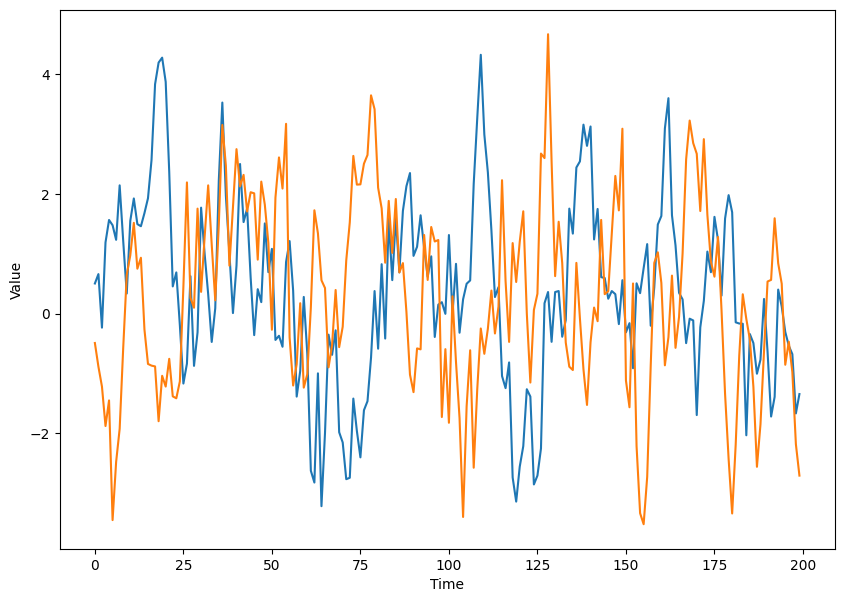
\includegraphics[scale=0.35]{./images/naive_ou.png}
\end{center}
Here we can see that the stochastic process is much more contained within a range, and is thus mean-reverting.

\end{spacing}

\section{Derivation of the Gradient for Non-linear Programming}
We optimize for the variable $\theta$. We get following base function.
\begin{gather*}
    X_{t + 1} = X_{t} + -\theta(X_{t} - \mu)e + \mathcal{N}(0, \sigma^{2}) \\
\end{gather*}
We must get the objective function which is thre mean squared error in terms of $\theta$.
We consider the the values to be in a pre-computed list $\mathcal{X}$, where $\mathcal{X}_{1}, \mathcal{X}_{2}, \cdots, \mathcal{X}_{n} \in \mathcal{X}$
\begin{gather*}
    MSE = \frac{1}{T} \sum_{i = 1}^{T} \mathcal{X}_{i} = \frac{1}{T} \sum_{i = 1}^{T} X_{i} + -\theta(X_{t} - \mu)e + \mathcal{N}(0, \sigma^{2})
\end{gather*}

\section{Least Squares Regression for Mean-reverting Parameter}
\begin{gather*}
    \mathcal{X}_{t + 1} = \mathcal{X}_{t} - \theta (X_{t} - \mu)e + \mathcal{N}(0, \sigma^{2}) \\
    \mathcal{X}_{t + 1} - \mathcal{X}_{t} - \mathcal{N}(0, \sigma^{2}) = -\theta (X_{t} - \mu)e  \\
    \frac{- \mathcal{X}_{t + 1} + \mathcal{X}_{t} + \mathcal{N}(0, \sigma^{2})}{e(X_{t} - \mu)} = \theta
\end{gather*}

For now, we can disregard the normally-distributed Wiener process term.

\end{document}
